\documentclass[11pt]{article}
\usepackage{listings}
\usepackage{tikz}
\usepackage{url}
\usepackage{alltt}
%\usepackage{algorithm2e}
\usetikzlibrary{arrows,automata,shapes,decorations.pathreplacing,positioning}
\tikzstyle{block} = [rectangle, draw, fill=blue!20, 
    text width=2.5em, text centered, rounded corners, minimum height=2em]
\tikzstyle{bw} = [rectangle, draw, fill=blue!20, 
    text width=3.5em, text centered, rounded corners, minimum height=2em]

\newcommand{\handout}[5]{
  \noindent
  \begin{center}
  \framebox{
    \vbox{
      \hbox to 5.78in { {\bf ECE459: Programming for Performance } \hfill #2 }
      \vspace{4mm}
      \hbox to 5.78in { {\Large \hfill #5  \hfill} }
      \vspace{2mm}
      \hbox to 5.78in { {\em #3 \hfill #4} }
    }
  }
  \end{center}
  \vspace*{4mm}
}

\newcommand{\lecture}[4]{\handout{#1}{#2}{#3}{#4}{Lecture #1}}
\topmargin 0pt
\advance \topmargin by -\headheight
\advance \topmargin by -\headsep
\textheight 8.9in
\oddsidemargin 0pt
\evensidemargin \oddsidemargin
\marginparwidth 0.5in
\textwidth 6.5in

\parindent 0in
\parskip 1.5ex
%\renewcommand{\baselinestretch}{1.25}

% http://gurmeet.net/2008/09/20/latex-tips-n-tricks-for-conference-papers/
\newcommand{\squishlist}{
 \begin{list}{$\bullet$}
  { \setlength{\itemsep}{0pt}
     \setlength{\parsep}{3pt}
     \setlength{\topsep}{3pt}
     \setlength{\partopsep}{0pt}
     \setlength{\leftmargin}{1.5em}
     \setlength{\labelwidth}{1em}
     \setlength{\labelsep}{0.5em} } }
\newcommand{\squishend}{
  \end{list}  }
% http://gurmeet.net/2008/09/20/latex-tips-n-tricks-for-conference-papers/
\newenvironment{itemizep}{
 \begin{itemize}
  \setlength{\itemsep}{0pt}
  \setlength{\parsep}{3pt}
  \setlength{\topsep}{3pt}
  \setlength{\partopsep}{0pt}
  \setlength{\leftmargin}{1.5em}
  \setlength{\labelwidth}{1em}
  \setlength{\labelsep}{0.5em} }
 {\end{itemize}}
\lstdefinelanguage{JavaScript}{
  keywords={typeof, new, true, false, catch, function, return, null, catch, switch, var, if, in, while, do, else, case, break},
  keywordstyle=\color{blue}\bfseries,
  ndkeywords={class, export, boolean, throw, implements, import, this},
  ndkeywordstyle=\color{darkgray}\bfseries,
  identifierstyle=\color{black},
  sensitive=false,
  comment=[l]{//},
  morecomment=[s]{/*}{*/},
  commentstyle=\color{purple}\ttfamily,
  stringstyle=\color{red}\ttfamily,
  morestring=[b]',
  morestring=[b]"
}
\begin{document}

\lecture{27 --- March 13, 2015}{Winter 2015}{Patrick Lam}{version 1}
Today's lecture is about lies your profiler tells you. We'll talk about two types
of lies today: lies about calling context, and lies about cost attribution.

\section*{Lies about Calling Context}
We'll start by talking about gprof and callgrind/KCacheGrind.

Some profiler results are real.  Other results are interpolated, and
perhaps wrong. Who can we trust?

The reference for this part of the lecture is a blog post by Yossi Kreinin,
found at \url{http://www.yosefk.com/blog/how-profilers-lie-the-cases-of-gprof-and-kcachegrind.html}.

\paragraph{Running Example.} Consider the following code.

\begin{lstlisting}
void work(int n) {
  volatile int i=0; //don't optimize away
  while(i++ < n);
}
void easy() { work(1000); }
void hard() { work(1000*1000*1000); }
int main() { easy(); hard(); }
\end{lstlisting}

We see that there is a worker function whose runtime depends on its input.
Function {\tt easy} calls the worker function with a small input, and {\tt hard} calls
it with a large input. Profiling yields:
\begin{alltt}
[plam@lynch L27]\$ gprof ./try gmon.out
Flat profile:

Each sample counts as 0.01 seconds.
  \%   cumulative   self              self     total           
 time   seconds   seconds    calls  ms/call  ms/call  name    
101.30      1.68     1.68        2   840.78   840.78  work
  0.00      1.68     0.00        1     0.00  {\bf 840.78}  easy
  0.00      1.68     0.00        1     0.00  {\bf 840.78}  hard
\end{alltt}
%$
Most of the profiler output is just fine. But there are lies in the
``total ms/call'' column. The call to {\tt easy} takes about 0 seconds,
while that to {\tt hard} takes 1.68s. Less importantly, the total ms/call for
{\tt work} is indeed an average, but that hides the variance between runtimes.

\paragraph{Why?} To make any sense of the lies, we need to understand how {\tt gprof} works.
It uses two standard-library functions: {\bf profil()} and {\bf mcount()}.

\squishlist
\item {\bf profil()}: asks glibc to record which instruction 
  is currently executing (100$\times$/second).
\item {\bf mcount()}: records call graph edges; called by {\tt -pg} instrumentation.
\squishend

Hence, {\bf profil} information is statistical, while {\bf mcount}
information is exact.  Bringing that information back to the profiler
output columns, we can see that the ``calls'' column is reliable; the
``self seconds'' column is sampled, but reasonably accurate here; and
the ``total ms/call'' is interpolated, and we deceived it in this
contrived example. How is that?

gprof sees:
\squishlist
    \item a total of 1.68s in {\tt work};
    \item 1 call to {\tt work} from {\tt easy}; and
    \item 1 call to {\tt work} from {\tt hard}.
\squishend
All of these numbers are reliable. However, gprof draws the unreliable inference that
both {\tt easy}, {\tt hard} cause 840ms of {\tt work} time.

This is wrong. {\tt work} takes 1000000$\times$ longer when called from {\tt hard}!

The following results from gprof are suspect:
\squishlist
  \item contribution of children to parents;
  \item total runtime spent in self+children;
  \item etc.
\squishend

\paragraph{When are call graph edges right?}
Two cases:
    \begin{itemize}
    \item functions with only one caller
      (e.g. {\tt f()} only called by {\tt g()}); or,
    \item functions which always take the same time to complete
      (e.g. {\tt rand()}).
    \end{itemize}

On the other hand, results for any function whose running time depends on its inputs,
and which is called from multiple contexts, are sketchy.

\subsection*{callgrind/KCacheGrind}
Next, we'll talk about callgrind/KCacheGrind.  callgrind is part of
valgrind, and runs the program under an x86 JIT.  KCacheGrind is a
frontend to callgrind. callgrind gives better information, but imposes
more overhead.

\newpage
KCacheGrind works properly on the earlier running example:

\begin{center}
  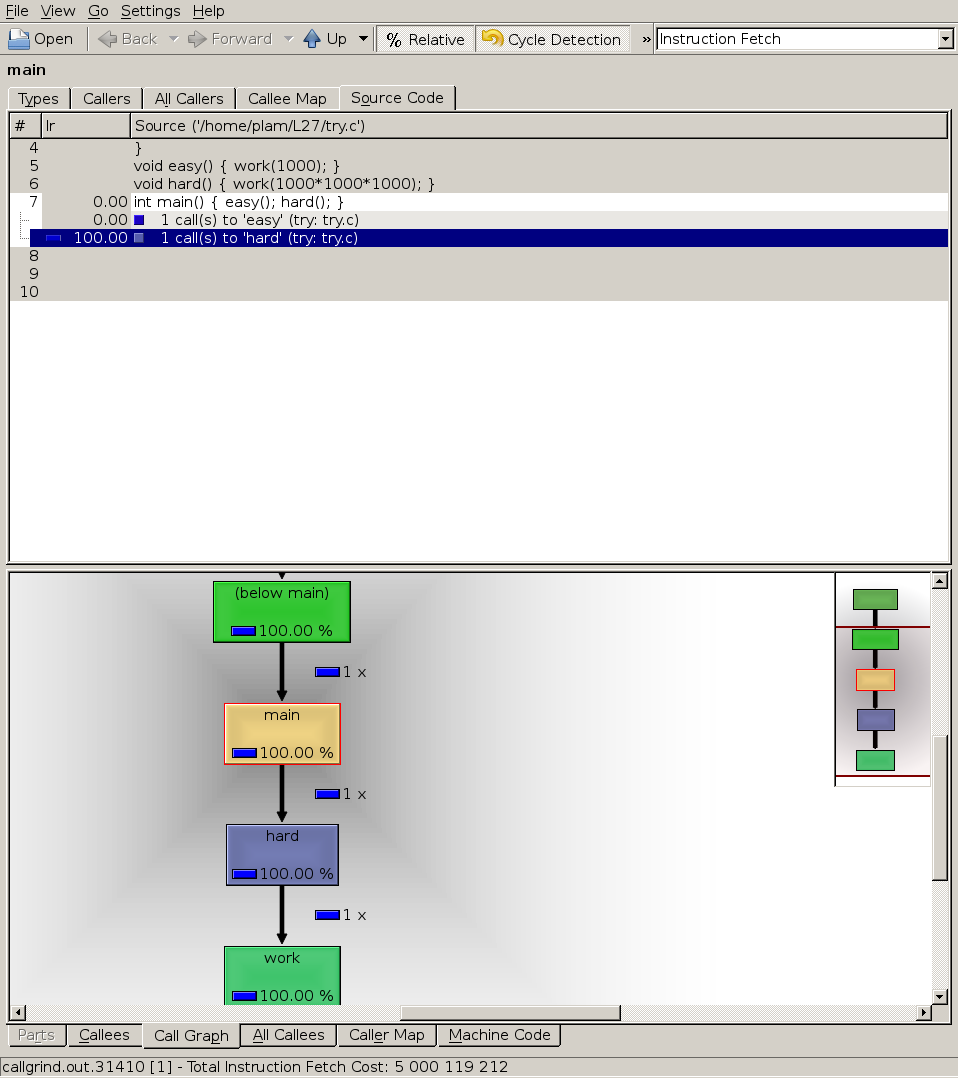
\includegraphics[width=.4\textwidth]{L27/kcachegrind}
\end{center}

It properly reports that {\tt hard} takes all the time.
But we can still deceive it.

\paragraph{More Complex Example.} Let's look at this example.

\begin{minipage}{.4\textwidth}
\begin{lstlisting}[basicstyle=\scriptsize]
void worker1(int n) {
  volatile int i=0;
  while(i++<n);
}
void worker2(int n) {
  volatile int i=0;
  while(i++<n);
}
void manager(int n1, int n2) {
  worker1(n1);
  worker2(n2);
}
\end{lstlisting}
\end{minipage}
\begin{minipage}{.4\textwidth}
\begin{lstlisting}[basicstyle=\scriptsize]
void project1() {
  manager(1000, 1000000);
}
void project2() {
  manager(1000000, 1000);
}
int main() {
  project1();
  project2();
}
\end{lstlisting}
\end{minipage}

Now, {\tt worker2} takes all the time in {\tt project1},
and {\tt worker1} takes all the time in {\tt project2}.

Let's see how KCacheGrind does on this example.

\begin{center}
  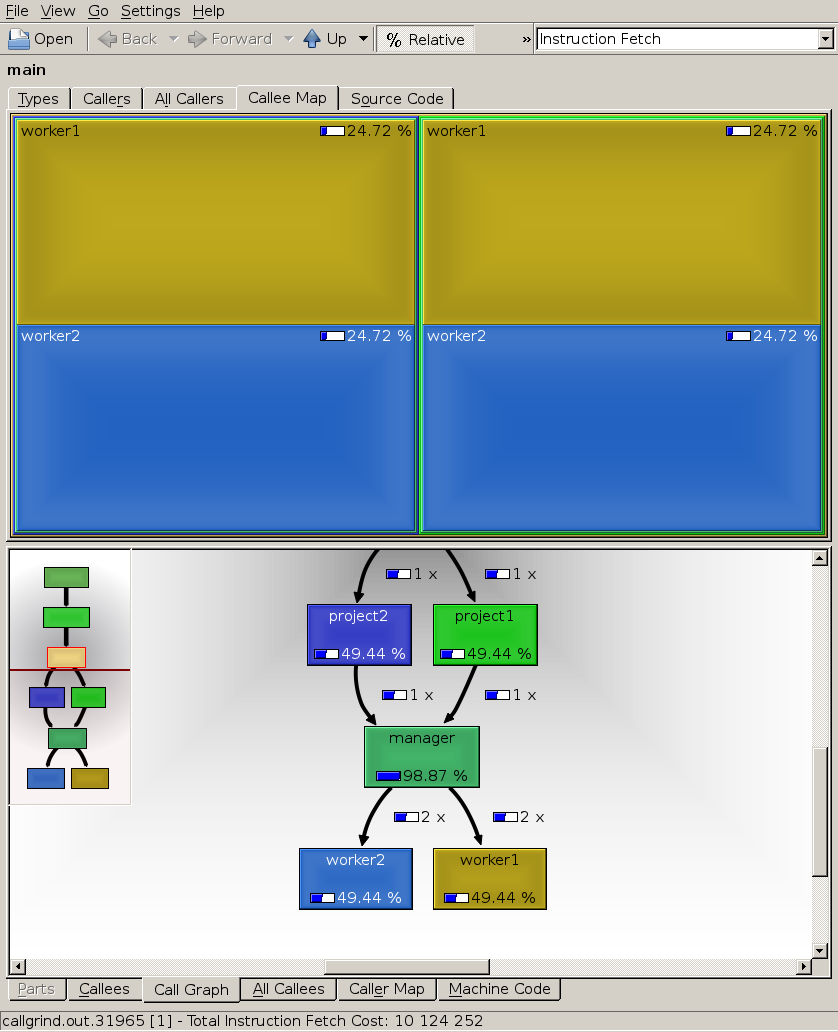
\includegraphics[width=.25\textwidth]{L27/kcachegrind2}
\end{center}


The call graph, on the bottom, shows that 
{\tt worker1} and {\tt worker2} do each take about 50\% of time.
So do {\tt project2} and {\tt project1}. This is fine.
(I think gprof would correctly interpolate that too.)

However, KCacheGrind also lies, in the report on top. It is saying
that {\tt worker1} and {\tt worker2} doing half the work in each
project.  That's not what the code says. Why is it lying?

\squishlist
\item gprof reports time spent in {\tt f()} and {\tt g()},
and how many times {\tt f()} calls {\tt g()}.
\item callgrind also reports 
time spent  in {\tt g()} when called from {\tt f()}, i.e. some calling-context information.
\item callgrind does \emph{not} report time spent in {\tt g()} when
     called from {\tt f()} when called from {\tt h()}.
     We don't get the {\tt project1} to {\tt manager} to {\tt worker1} link.
     (We have Edges but need Edge-Pairs).
\squishend

\paragraph{Summary.} We've seen that some profiler results are exact;
some results are sampled; and some results are interpolated.

If you understand the tool, you understand where it can go
wrong.

Understand your tools!

\section*{Lies from Metrics}
While app-specific metrics can lie too, mostly we'll talk about CPU
perf counters today.

The reference here is a blog post by Paul Khuong, found at 
\url{http://www.pvk.ca/Blog/2014/10/19/performance-optimisation-~-writing-an-essay/}.

This goes back to {\tt mfence}, which we've seen before. It is used, for instance, in
spinlock implementations. Khuong found that his profiles said that spinlocking didn't take much time.
But empirically: eliminating spinlocks = better than expected! Hmm.

The next step is (as we do in this course) to create microbenchmarks to better understand what's
going on. The microbenchmark contained memory accesses to uncached locations, or computations,
surrounded by store pairs/mfence/locks. He used perf to evaluate the impact of mfence vs lock.

{\scriptsize
\begin{lstlisting}
# for locks:
$ perf annotate -s cache_misses
[...]
    0.06 :        4006b0:       and    %rdx,%r10
    0.00 :        4006b3:       add    $0x1,%r9
    ;; random (out of last level cache) read
    0.00 :        4006b7:       mov    (%rsi,%r10,8),%rbp
   30.37 :        4006bb:       mov    %rcx,%r10
    ;; foo is cached, to simulate our internal lock
    0.12 :        4006be:       mov    %r9,0x200fbb(%rip)
    0.00 :        4006c5:       shl    $0x17,%r10
    [... Skipping arithmetic with < 1% weight in the profile]
    ;; locked increment of an in-cache "lock" byte
    1.00 :        4006e7:       lock incb 0x200d92(%rip)
   21.57 :        4006ee:       add    $0x1,%rax
    [...]
    ;; random out of cache read
    0.00 :        400704:       xor    (%rsi,%r10,8),%rbp
   21.99 :        400708:       xor    %r9,%r8
    [...]
    ;; locked in-cache decrement
    0.00 :        400729:       lock decb 0x200d50(%rip)
   18.61 :        400730:       add    $0x1,%rax
    [...]
    0.92 :        400755:       jne    4006b0 <cache_misses+0x30>
\end{lstlisting}
}

We can see that in the lock situation, reads take 30 + 22 = 52\% of runtime,
while locks take 19 + 21 = 40\% of runtime.

{\scriptsize
\begin{lstlisting}
# for mfence:
$ perf annotate -s cache_misses
[...]
    0.00 :        4006b0:       and    %rdx,%r10
    0.00 :        4006b3:       add    $0x1,%r9
    ;; random read
    0.00 :        4006b7:       mov    (%rsi,%r10,8),%rbp
   42.04 :        4006bb:       mov    %rcx,%r10
    ;; store to cached memory (lock word)
    0.00 :        4006be:       mov    %r9,0x200fbb(%rip)
    [...]
    0.20 :        4006e7:       mfence 
    5.26 :        4006ea:       add    $0x1,%rax
    [...]
    ;; random read
    0.19 :        400700:       xor    (%rsi,%r10,8),%rbp
   43.13 :        400704:       xor    %r9,%r8
    [...]
    0.00 :        400725:       mfence 
    4.96 :        400728:       add    $0x1,%rax
    0.92 :        40072c:       add    $0x1,%rax
    [...]
    0.36 :        40074d:       jne    4006b0 <cache_misses+0x30>
\end{lstlisting}
}
Looks like the reads take 85\% of runtime,
while the mfence takes 15\% of runtime.

Metrics lie, though, and when you focus on the metrics as opposed to what you
actually care about, it's easy to be led astray.

In this case, what we actually care about is the total \# of cycles.

    \begin{tabular}{lr}
    No atomic/fence:& 2.81e9 cycles\\
    lock inc/dec: & 3.66e9 cycles\\
    mfence: & 19.60e9 cycles
    \end{tabular}

That 15\% number is a total lie.
Profilers, even using CPU expense counts, drastically underestimate the impact of mfence,
and overestimate the impact of locks.

This is because mfence causes a pipeline flush, and the resulting 
costs get attributed to instructions being flushed, not to the mfence itself.

\paragraph{Summary} We saw a bunch of lies today: calling-context lies and perf attribution
lies. To avoid being bitten by lies, remember to focus on the metric you actually care about,
and understand how your tools work.

\end{document}
